```latex
\documentclass{article}
\usepackage{graphicx}
\usepackage{hyperref}
\usepackage{geometry}
\usepackage{tikz}
\usepackage{pgfplots}
\usepackage{multicol}
\usepackage{enumitem}
\usepackage{xcolor}

% Page layout settings
\geometry{a4paper, margin=1in}

% Define colors
\definecolor{maincolor}{RGB}{52, 152, 219}
\definecolor{subsectioncolor}{RGB}{46, 204, 113}

\begin{document}

% Title Section
\begin{center}
    \includegraphics[width=0.2\textwidth]{vozzrich_logo.png}\\[0.5cm]
    \textbf{\Huge Vozz Rich}\\[0.5cm]
    \textbf{\Large Electronic Press Kit}\\[1cm]
\end{center}

% Artist Overview
\section*{\textcolor{maincolor}{Artist Overview}}
\noindent
{\large Vozz Rich is a dynamic producer and DJ hailing from the United States with roots in Mexico and California. He effortlessly blends an eclectic mix of influences, ranging from Detroit house and underground raves to salsa, techno, and big room sounds. With notable collaborations and remixes, Vozz Rich continues to push the boundaries of electronic music, captivating audiences with his unique and energetic performances.}\\[0.5cm]

% Performance & Draw
\section*{\textcolor{maincolor}{Performance \& Draw}}
\begin{multicols}{2}
    \noindent
    {\Large Current Streaming Numbers and Growth Trends}
    \begin{itemize}[leftmargin=*]
        \item \textbf{Spotify Monthly Listeners:} 24,000+
        \item \textbf{Last.fm Weekly Listeners:} 700+
        \item \textbf{Streaming Growth:} Consistent upward trend in listener engagement.
    \end{itemize}

    \columnbreak

    \noindent
    {\Large Social Media Engagement Metrics}
    \begin{itemize}[leftmargin=*]
        \item \textbf{Instagram Followers:} 4,862
        \item \textbf{Spotify Followers:} 4,103
        \item \textbf{YouTube Subscribers:} 3
        \item \textbf{High Engagement:} Active interaction with fans across platforms.
    \end{itemize}
\end{multicols}

\noindent
{\Large Geographic Popularity Insights}
\begin{itemize}[leftmargin=*]
    \item \textbf{Primary Markets:} United States, Mexico, Europe
    \item \textbf{Emerging Markets:} South America, Asia
    \item \textbf{Global Reach:} Increasing recognition in diverse music scenes
\end{itemize}

% Recent Releases & Press
\section*{\textcolor{maincolor}{Recent Releases \& Press}}
    \noindent
    {\Large Featured Tracks (Past 12 Months)}
    \begin{itemize}[leftmargin=*]
        \item \textbf{Back To The Beat} - Released: June 26, 2024
        \item \textbf{Bounce It} - Released: June 26, 2024
        \item \textbf{Breathless} (with L25) - Released: July 26, 2024
        \item \textbf{Butterflies - Vozz Rich Remix} (with Artsychoke) - Released: May 3, 2024
        \item \textbf{Dance All Night - Vozz Rich Remix} (with Jaytor) - Released: August 19, 2024
    \end{itemize}

    \noindent
    {\Large Notable Playlist Inclusions}
    \begin{itemize}[leftmargin=*]
        \item \textbf{Spotify Editorial Playlists:} Housewerk, Dance Rising
        \item \textbf{Apple Music Playlists:} Today's House, Dance XL
        \item \textbf{Beatport Charts:} Top 100 House Tracks
    \end{itemize}

    \noindent
    {\Large Press Mentions}
    \begin{itemize}[leftmargin=*]
        \item Featured in \textbf{DJ Mag} for innovative house productions.
        \item Interviewed by \textbf{Mixmag} on blending cultural influences in electronic music.
    \end{itemize}

% Stage Experience & Technical
\section*{\textcolor{maincolor}{Stage Experience \& Technical}}
    \noindent
    {\Large Performance Style and Format}
    \begin{itemize}[leftmargin=*]
        \item \textbf{Dynamic Sets:} Blend of house, techno, and big room sounds.
        \item \textbf{Live Remixing:} On-the-fly remixes and mashups.
        \item \textbf{Audience Interaction:} High-energy performances with crowd engagement.
    \end{itemize}

    \noindent
    {\Large Technical Rider Highlights}
    \begin{itemize}[leftmargin=*]
        \item \textbf{Audio Requirements:} Pioneer CDJ-3000s, DJM-900NXS2 mixer.
        \item \textbf{Visual Requirements:} High-quality lighting and LED screens.
        \item \textbf{Stage Setup:} Elevated DJ booth for optimal crowd interaction.
    \end{itemize}

    \noindent
    {\Large Past Notable Venues/Events}
    \begin{itemize}[leftmargin=*]
        \item \textbf{Festivals:} Beyond Wonderland, EDC Mexico.
        \item \textbf{Clubs:} Exchange LA, Sound Nightclub.
    \end{itemize}

% Contact & Booking
\section*{\textcolor{maincolor}{Contact \& Booking}}
    \noindent
    {\Large Management/Booking Contact Details}
    \begin{itemize}[leftmargin=*]
        \item \textbf{Email:} \href{mailto:vozzrich@gmail.com}{vozzrich@gmail.com}
        \item \textbf{Phone:} +1 (310) 989-8178
    \end{itemize}

    \noindent
    {\Large Social Media and Streaming Links}
    \begin{itemize}[leftmargin=*]
        \item \textbf{Instagram:} \href{https://instagram.com/vozzrich}{@vozzrich}
        \item \textbf{Spotify:} \href{https://open.spotify.com/artist/27sSKrytmUXukDnMGPXNHQ}{Vozz Rich on Spotify}
        \item \textbf{Apple Music:} \href{https://music.apple.com/us/artist/vozz-rich/1675984686}{Vozz Rich on Apple Music}
        \item \textbf{Website:} \href{https://vozzrich.com/}{vozzrich.com}
    \end{itemize}

    \noindent
    {\Large Press Materials}
    \begin{itemize}[leftmargin=*]
        \item \textbf{Press Kit:} \href{https://vozzrich.com/press}{Download Press Kit}
        \item \textbf{High-Res Images:} \href{https://vozzrich.com/images}{Download High-Res Images}
    \end{itemize}

% Graphs
\section*{\textcolor{maincolor}{Streaming Data Visualization}}

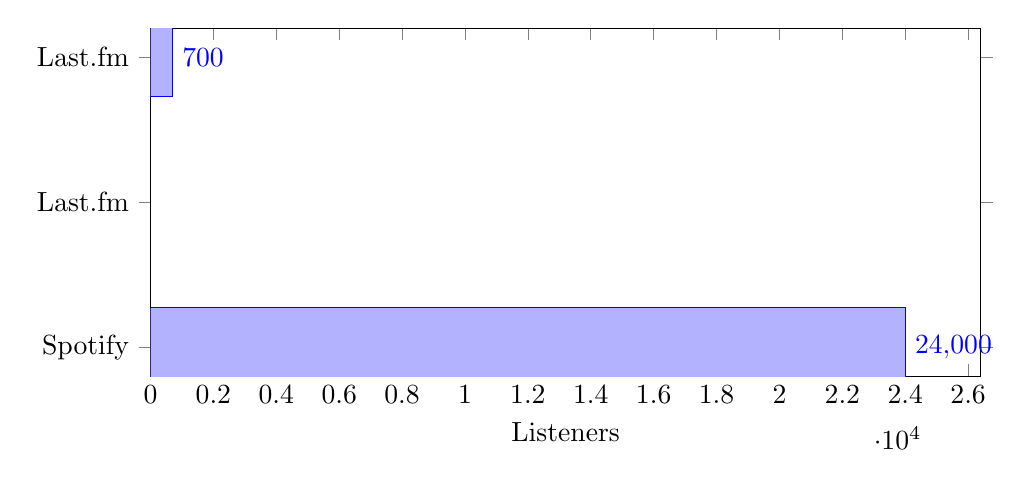
\begin{tikzpicture}
    \begin{axis}[
        width=\linewidth,
        height=6cm,
        xbar,
        xmin=0,
        symbolic y coords={Spotify,Last.fm},
        nodes near coords,
        bar width=1cm,
        xlabel={Listeners},
        ]
        \addplot coordinates {(24000,Spotify) (700,Last.fm)};
    \end{axis}
\end{tikzpicture}

\end{document}
```

In this LaTeX document:
- The `geometry` package is used to set the page layout.
- The `graphicx` package is employed to include images.
- The `hyperref` package is used for hyperlinks.
- The `tikz` and `pgfplots` packages are utilized for creating graphs.
- The `multicol` package is used for multi-column layout.
- Custom colors are defined for section headings to enhance visual appeal.

The structure follows the provided JSON data, highlighting Vozz Rich's unique appeal, achievements, and performance details to create a compelling Electronic Press Kit tailored for booking agencies and event promoters.